%!TEX root=../../../main.tex

The first considered use-case is one that originated on CDS. Here, the record
commenting facilities of Invenio are often employed by the high-energy physics
collaborations in order to review new papers in their pre-publication stage.
These collaborations use special workflows with multiple commenting rounds for
restricted drafts, necessary for amending potential issues before making
research results public \cite{ref:ludmila}.

In order to reference specific parts of the discussed papers, reviewers often
use a format similar to the following:
  \begin{itemize}
      \item \textit{``P1 - equation system is not presumed''}: a correction
          targeting the first page of the draft.
      \item \textit{``P1/L143 - equation system is not presumed''}: a variation
        of the above which also states the targeted text line.
      \item \textit{``Fig. 2 - equation system is not presumed''}: a comment on
        a figure.
      \item \textit{``P1, E2 - equation system is not presumed''}: a comment on
        Equation 2 on the first page.
  \end{itemize}
This format is also employed when the original paper authors respond to the
corrections, as shown in Fig. \ref{fig:comments}.

\begin{figure}[p]
  \centering
  \fbox{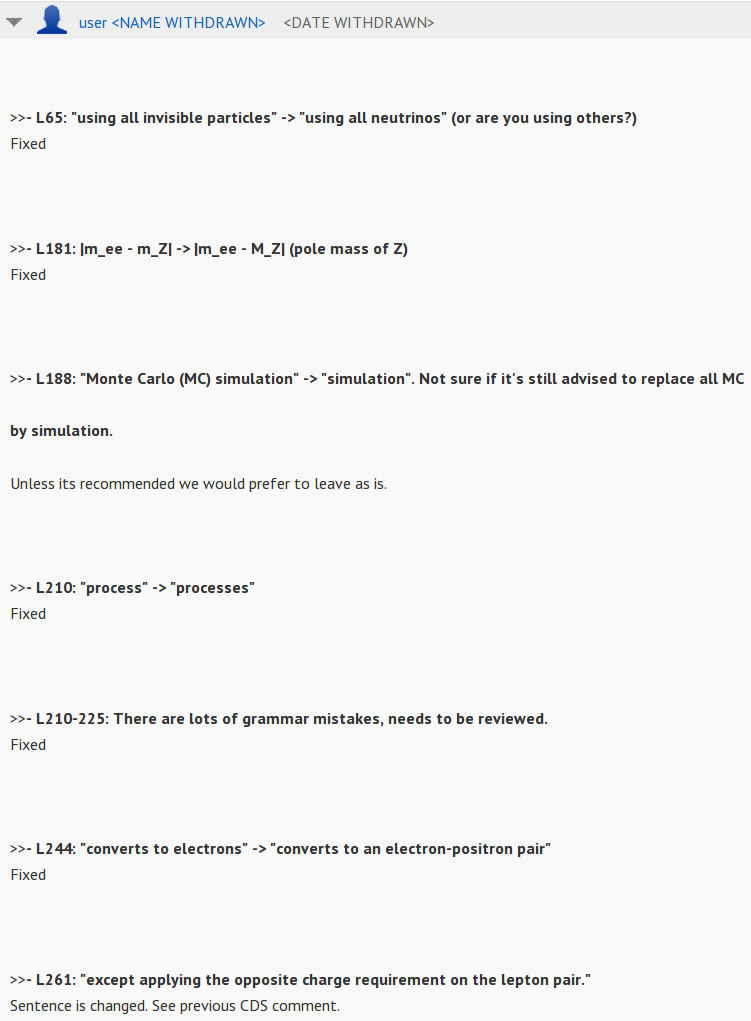
\includegraphics[scale=0.55]{static/img/comments.png}}
  \caption[Example of comments during the paper review phase on CDS]
          {Example of comments during the paper review phase on CDS. The author
           of a paper responds to corrections by referencing text line numbers.}
  \label{fig:comments}
\end{figure}

While being easy to use and clear regarding the corrections, this method also
presents a number of issues:
  \begin{enumerate}
    \item Non-standardised: even within the same commenting round of one draft,
      reviewers may use different variations of the markup; for example, to
      reference the first page, both ``P1'' and ``Pag1'' could be employed.
    \item Difficult to follow and aggregate: this issue emerged from the
      limitations of Invenio's commenting system which was not purposed for such
      structured input. Namely, both targeted remarks and free textual content
      could be combined in single comments, impeding reviewers from quickly
      identifying the required corrections to be made. Moreover, as commenting
      rounds can consist of hundreds of comments coming from multiple reviewers,
      aggregation is further hindered. For example, in a restricted CDS review
      round, we have identified over one thousand targeted remarks in 180
      comments coming from fifty persons.
  \end{enumerate}
Thus, a solution for solving these issues, while preserving the reviewing
workflow to which the end-users got accustomed to was required.

Aside from pre-publication reviews, such targeted notes could also be seen
useful for annotating resources (textual, multimedia or other formats). While
standard comments are sufficient for discussing general aspects regarding the
content, allowing annotations on various elements such as pages, figures or
paragraphs could prove useful for enriching the content and facilitating its
dissemination. Moreover, although comments often include a social aspect,
annotations could also be used in a private manner, for each user's self study.

\newpage

Another requirement emerges from the need to consolidate a number of features
present in Invenio and its deployed variants (CDS, INSPIRE) which share a number
of similarities:
\begin{enumerate}
  \item Comments and reviews: allow general remarks on records; reviews include
    a ``\textit{star score}''.
  \item Tags: a new feature to be released in the next major version of Invenio,
    allows users to add brief annotations to records mainly in order to
    organise and categorise them. Can be public, personal to each user, or
    shared between groups.
  \item Baskets: allow users to create collections of records and annotate them.
    Similar to tags, can be private or shared.
\end{enumerate}

Apart from these general Invenio features, certain deployments integrate their
own homologous functionalities. One example is INSPIRE, which implemented a
custom form for allowing users to suggest corrections for the citation list of
papers as the one in Fig. \ref{fig:inspire}. This can be seen as a particular
use-case of the record document review practices previously described, in which
only the reference list is considered.

\begin{figure}[!ht]
  \centering
  \fbox{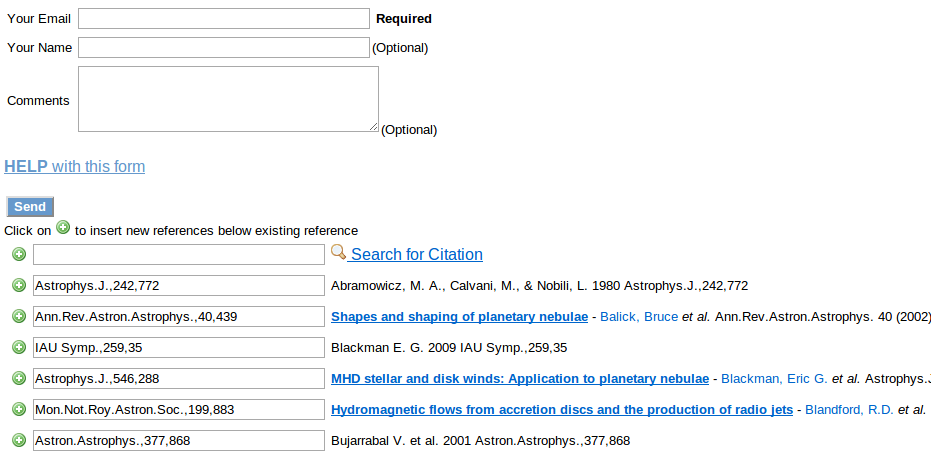
\includegraphics[scale=0.49]{static/img/inspire.png}}
  \caption[Reference correction form as implemented by INSPIRE.]
          {Reference correction form as implemented by INSPIRE. Users are
           invited to suggest amends, a structured form being used for guiding
           data input.}
  \label{fig:inspire}
\end{figure}

Finally, the high demand for a metadata dissemination facility has motivated
this project. As mentioned, Invenio already includes features enabling record
harvesting in compliance with the OAI protocol, but currently does not
implement any specific mechanism for exporting user-generated metadata, which
can provide more context to consumers.
